\documentclass[a4paper,11pt,dvipsnames, oneside]{memoir} %openright if a more "booklike report is wished, %,twoside,openany

\usepackage{listings}
\usepackage{color} %red, green, blue, yellow, cyan, magenta, black, white
\definecolor{mygreen}{RGB}{28,172,0} % color values Red, Green, Blue
\definecolor{mylilas}{RGB}{170,55,241}
\setlength\extrarowheight{2pt}
\usepackage{rotating}



\lstset{language=Matlab,%
	%basicstyle=\color{red},
	breaklines=true,%
	morekeywords={matlab2tikz},
	keywordstyle=\color{blue},%
	morekeywords=[2]{1}, keywordstyle=[2]{\color{black}},
	identifierstyle=\color{black},%
	stringstyle=\color{mylilas},
	commentstyle=\color{mygreen},%
	showstringspaces=false,%without this there will be a symbol in the places where there is a space
	numbers=left,%
	numberstyle={\tiny \color{black}},% size of the numbers
	numbersep=9pt, % this defines how far the numbers are from the text
	emph=[1]{for,end,break},emphstyle=[1]\color{red}, %some words to emphasise
	%emph=[2]{word1,word2}, emphstyle=[2]{style},    
}


%%%%% PACKAGES %%%%%%
\usepackage[utf8]{inputenc}
\usepackage{nomencl}
\usepackage{fixltx2e}						% Suscript i text
\usepackage{lastpage}						% Giver mulighed for "side x af y"
\usepackage{url}							% Giver mulighed for links i fodnote
\usepackage{array}
\usepackage{calc}
\usepackage{pgf}
\usepackage{mwe}	
\usepackage[nomessages]{fp}
\usepackage{cite}
%\usepackage{booktabs} 						% Punktopstilling til mufs bachelor
\usepackage{appendix}
\usepackage{lmodern}
%\usepackage[colorlinks=true,citecolor=green]{hyperref}

%%%%% TIKZ %%%%%
\usepackage{tikz}
\usetikzlibrary{circuits.ee.IEC,shapes,arrows,spy,positioning,snakes,plotmarks,backgrounds}
\usepackage[american voltages, american currents,siunitx,smartlabels]{circuitikz}
\usepackage{pgfplots}

%%%%% OVERSAETTELSE OG TEGNSAETNING %%%%%
%\usepackage[danish]{babel}					% Dokumentets sprog
\usepackage[T1]{fontenc}					% Output-indkodning af tegnsaet (T1)
\usepackage{ragged2e,anyfontsize}			% Justering af elementer
\usepackage{fixltx2e}						% Retter forskellige fejl i LaTeX-kernen
\usepackage{animate}		
%%%%% FIGURES AND TABLES %%%%%
\usepackage{pbox}							% Tvungne linjeskift i tabeller
\usepackage{tabularx}						% Tvungne linjeskift i tabeller
\usepackage{graphicx} 						% Haandtering af eksterne billeder (JPG, PNG, EPS, PDF)
\usepackage{graphics} % for pdf, bitmapped graphics files
\usepackage{eso-pic}						% Tilfoej billedekommandoer paa hver side
\usepackage{multirow}                		% Fletning af raekker og kolonner (\multicolumn og \multirow)
\usepackage{multicol}         	        	% Muliggoer output i spalter
\usepackage{rotating}						% Rotation af tekst med \begin{sideways}...\end{sideways}
\usepackage{colortbl} 						% Farver i tabeller (fx \columncolor og \rowcolor)
\usepackage{xcolor}							% Definer farver med \definecolor
\usepackage{flafter}						% Soerger for at floats ikke optraeder i teksten foer deres reference
\let\newfloat\relax 						% Justering mellem float-pakken og memoir
\usepackage{float}							% Muliggoer eksakt placering af floats, f.eks. \begin{figure}[H]
\graphicspath{{./figures/}}					% Saetter default grafik-sti
\usepackage{placeins}						% \FloatBarrier
\usepackage{wrapfig}


%%%%% MATEMATIK MED MERE %%%%%
\usepackage{amsmath,amssymb,stmaryrd} 		% Avancerede matematik-udvidelser
\usepackage{mathtools}						% Andre matematik- og tegnudvidelser
\usepackage{textcomp}                 		% Symbol-udvidelser
\usepackage{rsphrase}						% Kemi-pakke til RS-saetninger,
\usepackage[version=3]{mhchem} 				% Kemi-pakke til flot og let notation af formler
\usepackage{siunitx}						% Flot og konsistent praesentation af tal og enheder med \si{enhed} og \SI{tal}{enhed}
%\sisetup{locale=DE}						% Opsaetning af \SI (DE for komma som decimalseparator) 
\sisetup{output-decimal-marker = {.}}		% Bruges ved engelske rapporter

%%%%% REFERENCES AND SOURCES %%%%%
\usepackage[danish]{varioref}				% Muliggoer bl.a. krydshenvisninger med sidetal (\vref)
\usepackage[numbers]{natbib}				% Udvidelse med naturvidenskabelige citationsmodeller
\usepackage{xr}								% Referencer til eksternt dokument med \externaldocument{<NAVN>}
\usepackage{glossaries}						% Terminologi- eller symbolliste (se mere i Daleifs Latex-bog)

%%%%% MISC. %%%%%%
\usepackage{titlesec}
\usepackage{epigraph}
\usepackage{lipsum}							% Dummy text \lipsum[..]
\usepackage[shortlabels]{enumitem}			% Muliggoer enkelt konfiguration af lister
\usepackage{pdfpages}						% Goer det muligt at inkludere pdf-dokumenter med kommandoen \includepdf[pages={x-y}]{fil.pdf}	
\pdfoptionpdfminorversion=6					% Muliggoer inkludering af pdf dokumenter, af version 1.6 og hoejere
\pretolerance=2500 							% Justering af afstand mellem ord (hoejt tal, mindre orddeling og mere luft mellem ord)
\usepackage[footnote,draft,english,silent,nomargin]{fixme}		

%%%%% MARGINS %%%%%%
\setlrmarginsandblock{3.5cm}{2.5cm}{*}		% \setlrmarginsandblock{Indbinding}{Kant}{Ratio}
\setulmarginsandblock{2.5cm}{3.0cm}{*}		% \setulmarginsandblock{Top}{Bund}{Ratio}
\checkandfixthelayout 						% Oversaetter vaerdier til brug for andre pakker

%%%%% AFSNITSFORMATERING %%%%%
\setlength{\parindent}{0mm}           		% Stoerrelse af indryk
\setlength{\parskip}{3mm}          			% Afstand mellem afsnit ved brug af double Enter
\linespread{1,1}							% Linie afstand
\titlespacing\section{0pt}{12pt plus 4pt minus 2pt}{0pt plus 2pt minus 2pt}
\titlespacing\subsection{0pt}{12pt plus 4pt minus 2pt}{0pt plus 2pt minus 2pt}
\titlespacing\subsubsection{0pt}{12pt plus 4pt minus 2pt}{0pt plus 2pt minus 2pt}

%%%%% BIBLIOGRAPHY %%%%%
%\bibpunct[,]{[}{]}{;}{a}{,}{,} 			% Definerer de 6 parametre ved Harvard henvisning
%\bibliographystyle{bibtex/harvard}			% Udseende af litteraturlisten.
\bibliographystyle{unsrtnat}



%%%%% TABLE OF CONTENTS %%%%%
\setsecnumdepth{subsection}		 			% Dybden af nummerede overkrifter 
\maxsecnumdepth{subsection}					% Dokumentklassens graense for nummereringsdybde
\settocdepth{section} 						% Dybden af indholdsfortegnelsen

%%%%% LISTS (ENUMERATE, ITEMIZE) %%%%%
\setlist{
  topsep=0pt,								% Vertikal afstand mellem tekst og listen
  itemsep=-1ex}								% Vertikal afstand mellem items
 
%%%%% HYPHENATION %%%%%
\usepackage{microtype}
%\renewcommand{\danishhyphenmins}{22} 		% bedre orddeling 
 
%%%%% "FIGUR" COMMAND %%%%%
\newcommand{\figur}[3]{
	\begin{figure}[htbp] \centering
		\includegraphics[width=#1\textwidth]{#2}
		\caption{#3}\label{fig:#2}
	\end{figure}} 
 
%%%%% "FIGURCROP" COMMAND %%%%%
\newcommand{\figurcrop}[8]{
	\begin{figure}[htbp] \centering
		\includegraphics[width=#1\textwidth, clip=true ,trim= #8cm #7cm #6cm #5cm]{#2}
		\caption{#3}\label{#4} % LEFT , BOTTOM , RIGHT , TOP
	\end{figure}} 

%%%%% VISUAL REFERENCES %%%%%
\usepackage[colorlinks]{hyperref}			% Danner klikbare referencer (hyperlinks) i dokumentet.
\hypersetup{colorlinks = true,				% Opsaetning af farvede hyperlinks (interne links, citeringer og URL)
   linkcolor = black,
   citecolor = black,
   urlcolor = blue}
\usepackage{bookmark}
\bookmarksetup{
  numbered,
  open,
  openlevel=0}								% Sætter dybden på ToC når pdf åbnes

%%%%% CAPTION SETTINGS %%%%%
\captionnamefont{\small\bfseries\itshape}	% Opsaetning af tekstdelen ('Figur' eller 'Tabel')
\captiontitlefont{\small}					% Opsaetning af nummerering
\captiondelim{. }							% Seperator mellem nummerering og figurtekst
\hangcaption								% Venstrejusterer flere-liniers figurtekst under hinanden
\captionwidth{\linewidth}					% Bredden af figurteksten
\setlength{\belowcaptionskip}{10pt}			% Afstand under figurteksten

%%%%% NAMING %%%%%
%\addto\captionsdanish{
%	\renewcommand\appendixname{Appendix}
	\renewcommand\contentsname{\scshape{Table of Contents}}
	\renewcommand\bibname{\scshape{References}}		
%	\renewcommand\appendixpagename{Appendix}
%	\renewcommand\appendixtocname{Appendix}
%	\renewcommand\cftchaptername{\chaptername~}		% Skriver "Kapitel" foran kapitlerne i ToC
%	\renewcommand\cftappendixname{\appendixname~}	% Skriver "Appendiks" foran appendiks i ToC
%}

%%%%% BEGIN CHAPTERSTYLE DESIGN %%%%%
\definecolor{numbercolor}{RGB}{0,0,0}		% Definerer en farve til brug til kapiteludseende
\newif\ifchapternonum

\makechapterstyle{OZTOPRAK-CHAPTER}{
  \renewcommand\beforechapskip{0pt}
  \renewcommand\printchaptername{}
  \renewcommand\printchapternum{}
  \renewcommand\printchapternonum{\chapternonumtrue}
  \renewcommand\chaptitlefont{\fontfamily{pbk}\fontseries{db}\fontshape{n}\fontsize{20}{35}\selectfont\raggedright}
  \renewcommand\chapnumfont{\fontfamily{pbk}\fontseries{m}\fontshape{n}\fontsize{0.5in}{0in}\selectfont\color{numbercolor}}  
  \renewcommand\printchaptertitle[1]{%
    \noindent
    \ifchapternonum
    \begin{tabularx}{\textwidth}{X}
    	{\let\\\newline\chaptitlefont \scshape{##1}\par} 
    \end{tabularx}
    \par\vskip-2.5mm\hrule
    \else
    \begin{tabularx}{\textwidth}{Xl}
    	\raisebox{-0pt}{\chapnumfont \thechapter} & {\hspace{0.5cm} \parbox[b]{\linewidth}{\chaptitlefont \scshape{##1}}}
    \end{tabularx}
    \par\vskip2mm\hrule
    \fi
  }
}
%%%%% END CHAPTERSTYLE DESIGN %%%%%

%%%%% BEGIN PAGESTYLE DESIGN %%%%%
\makepagestyle{OZTOPRAK-PAGE}
\makepsmarks{OZTOPRAK-PAGE}{%
	\createmark{chapter}{left}{shownumber}{}{. \ }
	\createmark{section}{right}{shownumber}{}{. \ }
	\createplainmark{toc}{both}{\contentsname}
	\createplainmark{lof}{both}{\listfigurename}
	\createplainmark{lot}{both}{\listtablename}
	\createplainmark{bib}{both}{\bibname}
	\createplainmark{index}{both}{\indexname}
	%\createplainmark{glossary}{both}{\glossaryname}
}
\nouppercaseheads												% Ingen Caps oenskes

%\makeevenhead{OZTOPRAK-PAGE}{\leftmark}{}{}				% {Name}{L}{C}{R}
%\makeoddhead{OZTOPRAK-PAGE}{}{}{ {\leftmark}  }	% {Name}{L}{C}{R}

\makeevenhead{OZTOPRAK-PAGE}{\leftmark}{}{}        % {Name}{L}{C}{R}
\makeoddhead{OZTOPRAK-PAGE}{\leftmark}{}{}    % {Name}{L}{C}{R}

\makeevenfoot{OZTOPRAK-PAGE}{}{\thepage\ }{}								% {Name}{L}{C}{R}
\makeoddfoot{OZTOPRAK-PAGE}{}{ \thepage\ }{}								% {Name}{L}{C}{R}

\makeheadrule{OZTOPRAK-PAGE}{\textwidth}{0.5pt}						% Tilfoejer en streg under sidehovedets indhold
%\makefootrule{OZTOPRAK-PAGE}{\textwidth}{0.5pt}{1mm}					% Tilfoejer en streg under sidefodens indhold

\copypagestyle{AAUchap}{OZTOPRAK-PAGE}								% Sidehoved for kapitelsider defineres som standardsider, men med blank sidehoved
\makeoddhead{AAUchap}{}{}{}
\makeevenhead{AAUchap}{}{}{}
\makeheadrule{AAUchap}{\textwidth}{0pt}
\aliaspagestyle{chapter}{AAUchap}				% Den ny style vaelges til at gaelde for chapters
%%%%% END PAGESTYLE DESIGN %%%%%						
													
%%%%% VALG AF CHAPTER OG PAGESTYLE %%%%%									
\chapterstyle{OZTOPRAK-CHAPTER}						% Valg af kapiteludseende				
\pagestyle{OZTOPRAK-PAGE}								% Valg af sidehoved og sidefod

%%%%% PART SETTINGS %%%%%
\aliaspagestyle{part}{empty}					% Fjerner sidetal på part sider
\renewcommand{\afterpartskip}{\vfil}

%%%%% INFO DECLARATIONS %%%%%%
\newcommand*{\supervisor}[1]{\def\supname{#1}}
\newcommand*{\thesistitle}[1]{\def\ttitle{#1}}
\newcommand*{\subtitle}[1]{\def\stitle{#1}}
\newcommand*{\examiner}[1]{\def\examname{#1}}
\newcommand*{\degree}[1]{\def\degreename{#1}}
\renewcommand*{\author}[1]{\def\authorname{#1}}
\newcommand*{\addresses}[1]{\def\addressname{#1}}
\newcommand*{\university}[1]{\def\univname{#1}}
\newcommand*{\department}[1]{\def\deptname{#1}}
\newcommand*{\group}[1]{\def\groupname{#1}}
\newcommand*{\faculty}[1]{\def\facname{#1}}
\newcommand*{\subject}[1]{\def\subjectname{#1}}
\newcommand*{\keywords}[1]{\def\keywordnames{#1}}

%--------------------------------
% code in latex
\usepackage{listings}
\usepackage{color}

\definecolor{mygreen}{RGB}{28,172,0} % color values Red, Green, Blue
\definecolor{mylilas}{RGB}{170,55,241}

\definecolor{dkgreen}{rgb}{0,0.6,0}
\definecolor{gray}{rgb}{0.5,0.5,0.5}
\definecolor{mauve}{rgb}{0.58,0,0.82}

\lstset{frame=tb,
  language=python,
  aboveskip=3mm,
  belowskip=3mm,
  showstringspaces=false,
  columns=flexible,
  basicstyle={\small\ttfamily},
  numbers=none,
  numberstyle=\tiny\color{gray},
  keywordstyle=\color{blue},
  commentstyle=\color{dkgreen},
  stringstyle=\color{mauve},
  breaklines=true,
  breakatwhitespace=true,
  tabsize=3
}

%\usepackage[utf8]{inputenc}
\usepackage{listingsutf8}
\lstset{language=Matlab,%
    %basicstyle=\color{red},
    breaklines=true,
    extendedchars=true,
    morekeywords={matlab2tikz},
    keywordstyle=\color{blue},%
    morekeywords=[2]{1}, keywordstyle=[2]{\color{black}},
    identifierstyle=\color{black},%
    stringstyle=\color{mylilas},
    commentstyle=\color{mygreen},%
    showstringspaces=false,%without this there will be a symbol in the places where there is a space
    numbers=left,%
    numberstyle={\tiny \color{black}},% size of the numbers
    numbersep=9pt, % this defines how far the numbers are from the text
    emph=[1]{for,end,break},emphstyle=[1]\color{blue}, %some words to emphasise
    %emph=[2]{word1,word2}, emphstyle=[2]{style},    
}
%%%% INFO %%%%%

\thesistitle{30550: Satellite Based Positioning}		% \ttitle
\subtitle{Report for assignment A-C}			% \stitle
\supervisor{Dr. Anna B. O. Jensen} 		% \supname
\author{Xiao Hu} 	% \authorname
\department{\textbf{National Space Institute}\\ Technical University of Denmark\\ Elektrovej Building 328, room 007\\ 2800 Kongens Lyngby\\ Denmark } % \deptname
\addresses{\url{www.space.dtu.dk}\\ \\ E-mail:~\url{xiahaa@space.dtu.dk}}


\examiner{EXAMNAME} 								% \examname
\degree{DEGREENAME} 								% \degreename
\university{Technical University of Denmark} 		% \univname
\addresses{} 										% \addressname
\subject{Subjectname} 								% \subjectname
\keywords{KEYWORDNAMES} 							% \keywordnames
\group{GROUPNAME} 									% \groupname
\faculty{FACNAME} 									% \facname


\begin{document}


%%%%% FRONTPAGE %%%%%
\begin{titlingpage}
	\thispagestyle{empty}
	\enlargethispage{1.3cm}
	\calccentering{\unitlength}
	\begin{adjustwidth}{\unitlength}{-\unitlength}
		\vspace*{-1.9cm}
%		\begin{textblock}{6.5}(5.5,0) %
%			
\includegraphics[width=\textwidth]{figures/tex_dtu_uk_a1_cmyk}
%		\end{textblock}
		\hspace{7cm}
		{\noindent 
\includegraphics[scale=1]{tex_dtu_uk_a1_cmyk}}
		
		\begin{raggedright}
			\vspace{\stretch{1}}
			{\huge\sffamily\authorname\\[2cm]}
			\begin{Spacing}{1.2}
				{\sffamily\HUGE\textbf{\ttitle}\\ [0.5cm]}
				{\sffamily\huge\textbf{\stitle}\\[1.5cm]}				
				{\sffamily\LARGE{\today}\\[2cm]}
			\end{Spacing}
			\vspace{\stretch{2}}
		\end{raggedright}
		\begin{raggedright}
			
\includegraphics[width=0.5\textwidth]{figures/tex_dtu_space_b_uk}%
%			\ifthenelse{\equal{\bCompanyLogo}{true}}{%
%				\begin{textblock}{3}(9,-0.85) %
%					\includegraphics[width=\textwidth]{gfx/CompanyLogo}
%				\end{textblock}
%			}{} % End if
		\end{raggedright}
	\end{adjustwidth}
%
	\clearpage

	\thispagestyle{empty}
	\enlargethispage{1.3cm}
	\calccentering{\unitlength}
	
	%\begin{adjustwidth}{\unitlength}{-\unitlength}
	%	\begin{raggedright}
	%		\vspace{\stretch{1}}
	%		{\huge\sffamily\authorname\\[2cm]}
	%		\begin{Spacing}{1.2}
	%			{\sffamily\HUGE\textbf{\ttitle}\\ [0.5cm]}
	%			{\sffamily\huge\textbf{\stitle}\\[1.5cm]}				
	%			{\sffamily\LARGE{Report Type, January YYYY}\\[2cm]}
	%		\end{Spacing}
	%		\vspace{\stretch{2}}
	%	\end{raggedright}
	%\end{adjustwidth}

	\clearpage
	\thispagestyle{empty}
	\calccentering{\unitlength}
	\begin{adjustwidth*}{\unitlength}{-\unitlength}
		\textbf{\ttitle, \stitle}
		\vspace{\stretch{1}}

		\noindent\textbf{Author(s):}\\
		\authorname

		\vspace{\stretch{1}}

		\noindent\textbf{Supervisor(s):}\\
		\supname

		\vspace{\stretch{8}}

		\noindent\deptname
		\vspace{\stretch{0.01}} \\
		\noindent\addressname
		\noindent \url{www.space.dtu.dk}\\ 
		\noindent \\ E-mail:~\url{xiahaa@space.dtu.dk}

		\vspace{\stretch{4}}

		%\noindent\ThElektroEmail

		%\vspace{\stretch{5}}
		%\rule{15.5cm}{.1pt} \\
		%\noindent{\renewcommand{\arraystretch}{2}\begin{tabular}{@{}lp{0.75\textwidth}}
		%	Release date:&	<date>\\
		%	Class:&		1 (Public)\\
		%	Edition:&   1. edition\\
		%	Comments:&	This report is a part of the requirements to achieve <De-gree/title> at Technical University of Denmark. The report represents <ECTS points> ECTS points.\\
		%	Rights:& <Owner>, <Year>
		%\end{tabular}}
	\end{adjustwidth*}
\end{titlingpage}


%%%%% FRONT MATTER %%%%%
\frontmatter 
%\newpage\thispagestyle{empty}\mbox{}	 % Creates blank page
%\chapter{Preface}
This report will present the procedures, results complished for assignments A-C which mainly includes transformation among common used coordinate frames and prediction of satellite position using Kepler theorem.
\chapter{Abstract}
This report will present the procedures, results accomplished for assignments A-C which mainly includes transformation among common used coordinate frames and prediction of satellite position using Kepler theorem. 
%\include{files/resume} 
%\chapter{Symbols}

\begin{table}[h]
\centering
%\caption{My caption}
%\label{my-label}
\begin{tabular}{lllll}
\textbf{Symbol} & \textbf{Unit} &  &  & \textbf{Definition} \\
R               & $\omega$      &  &  & Resistance          \\
                &               &  &  &                     \\
                &               &  &  &                    
\end{tabular}
\end{table}

Note: This section can be deleted if you do not need it – see section 3.4 for how to do it without messing up the headers. 

%%%%% ToC & FIXME %%%%%
\tableofcontents


%%%%% MAIN MATTER %%%%%%
\mainmatter
%\include{files/}
%\chapter{Assignment A: Geographic and Cartesian Coordinates}
The main objective of the assignment is to understand the two commonly used coordinate frames for satellite-based positioning and grasp the transformations between the two coordinate frames. 

\section{Theory}
According to~\cite{misra2006global}, the transformation from the ellipsoidal coordiante frame $(\phi,\ \lambda,\ h)$ to the earth-centered, earth-fixed (ECEF) Cartesian coordinate frame $(x,\ y,\ z)$ can be computed as follows:
\begin{align}
	N &= \frac{a^2}{(1-e^2sin^2{\phi})^{\frac{1}{2}}} \\
	\left[\begin{matrix}
		x \\
		y \\
		z \\
	\end{matrix}\right] &= \left[\begin{matrix}
	(N+h) cos(\phi)cos(\lambda) \\
	(N+h) cos(\phi)sin(\lambda) \\
	(N(1-e^2)+h)sin(\phi) \\
	\end{matrix}\right] 
\end{align}
where, $a$ is the semi-major axis of ellipsoid ($6378137.0$ m), $e$ is the eccentricity of the ellipsoid calculated by $e^2=2f-f^2$ with $f$ being the flattening ($\frac{1}{298.257223563}$). This transformation can be computed directly.

The backward transformation from the ECEF to the ellipsoidal coordinate frame is given by:
\begin{align}
	p &= \sqrt{x^2+y^2}\\
\left[
	\begin{matrix}
	\phi \\
	\lambda \\
	h \\
	\end{matrix}
\right] &= \left[
	\begin{matrix}
	atan(\frac{z}{p(1-e^2\frac{N}{N+h})}) \\
	atan(\frac{y}{x}) \\
	\frac{p}{cos(\phi)}-N \\
	\end{matrix}
\right]
\label{eq:1.1}
\end{align}
As can be seen~\eqref{eq:1.1}, the $h$ and $\phi$ correlate with each other, which means it can only be solved iteratively. 

\section{Tasks}
\begin{itemize}
	\item Implement a \textsc{Matlab} function for conversion from Latitude, Longitude, and Height to X, Y, and Z (in WGS84), and vice versa.
	\item Test with positions selected from the internet.
	\item Benchmark the results with results converted by the KMSTrans\footnote{\url{http://valdemar.kms.dk/trf/}} program.
\end{itemize}
\section{Code}
%\textcolor{red}{TODO: comment useless code. add necessary explanantion.}
Complementary functions: \\
\textbf{deg2rad: conversion from degree to radian}:
\lstinputlisting{../../assignment/utils/deg2rad.m}
\textbf{rad2deg: conversion from radian to degree}:
\lstinputlisting{../../assignment/utils/rad2deg.m}
\textbf{llhtoCartesian: conversion from latitide, longitude, altitude to Cartesian coordiantes}:
\lstinputlisting{../../assignment/utils/llhtoCartesian.m}
\textbf{cartesian2llh: conversion from Cartesian coordiantes to latitide, longitude, altitude}:
\lstinputlisting{../../assignment/utils/cartesian2llh.m}
\newpage
\lstinputlisting{../../assignment/ex1/ex1_coordinate_transformation.m}

\section{Experiments}
\subsection{Simple Test}
\subsubsection{Setup}
In this simple test, I manually selected several points among which there is one point representing the DTU 101, one point located on the equator, one point in the North pole and one in the South pole. Meanwhile, in order to validate the correctness given the inputs contain negative values, the fourth point contains negative values for latitude, longitude. Below is a table listing the four sample points.
\begin{table}[h]
	\centering
	\caption{Test cases}
	\label{tb1:test_cases}
	\begin{tabular}{c|c}
		\hline
		\textbf{ID} & \textbf{\{lati, longi, alti\}} \\ \hline
		1     &  \{55.78575300466123,12.525384183973078,40\}   \\ \hline
		2     & \{0,12.525384183973078,40\}     \\ \hline
		3 	  & \{90,0,40\} \\ \hline
		4	  & \{-90,-15,40\} \\ \hline
	\end{tabular}
\end{table}
\subsubsection{Result}
\begin{table}[h]
	\centering
	\caption{Backward Results}
	\label{tb2:btest_results}
	\begin{tabular}{c|c|c}
		\hline
		\textbf{$LLA$} & \textbf{$LLA$} by KMSTrans & \textbf{$RMS$} with KMSTrans \\ \hline
		\{55.7858, 12.5254, 40\}  & \{55.5626, 12.3355, 40\}   &  0.1692  \\ \hline
		\{0, 12.5254, 40\}  & \{0, 12.3355, 40\}   &  0.1096  \\ \hline
		\{90, 0, 40\}  & \{90.1478, 0, 40\}   &  0.0853  \\ \hline
		\{-90, -15, 40\}  & \{\textcolor{red}{N/A}\footnote{KMSTrans does not support this point.}\}   &  \textcolor{red}{N/A}  \\ \hline
	\end{tabular}
\end{table}
\begin{table}[h]
	\centering
	\caption{Backward Results}
	\label{tb3:fbtest}
	\begin{tabular}{c|c|c}
		\hline
		\textbf{Original $LLA$} & \textbf{Reconstructed $LLA$} & \textbf{$RMS$} \\ \hline
		\{55.7858, 12.5254, 40\}  & \{55.7858, 12.5254, 40\}   &  $2.1508e^{-09}$  \\ \hline
		\{0, 12.5254, 40\}  & \{0, 12.5254, 40\}   &  $5.377e^{-10}$  \\ \hline
		\{90, 0, 40\}  & \{90, 0, 40\}   &  0  \\ \hline
		\{-90, -15, 40\}  & \{-90, -15, 40\} &  $1.0256e^{-15}$ \\ \hline
	\end{tabular}
\end{table}
The forward result is shown in the following Table~\ref{tb1:ftest_results} where the first column lists the transformed $XYZ$ values, the second column lists the results from the KMSTrans website, the third column lists the error between the computed values and the results from the KMSTrans website in terms of Root-Mean-Squares $RMS$. \\
The backward result is shown in the Table~\ref{tb2:btest_results}, where the first column lists the re-computed values for latitude, longitude, altitude $LLA$, the second column lists the results from the KMSTrans website, the last column lists the error between the re-computed values and the refereed values from KMSTrans for latitude, longitude, altitude in terms of Root-Mean-Squares $RMS$.
\noindent% <-- important
\begin{sidewaystable}
%\begin{sidewaystable}[htbp]
\centering
\caption{Forward Results}
\label{tb1:ftest_results}
	\small
	\setlength\tabcolsep{2pt}
\begin{tabular}{c|c|c}	
	\hline
	\textbf{$XYZ$} & \textbf{$XYZ$} by KMSTrans & \textbf{$RMS$ with KMSTrans} \\ \hline
	\{3509064.2531, 779572.0321, 5251099.25\}  & \{3509064.253, 779572.032, 5251099.25\}   &  $8.1650e^{-05}$  \\ \hline
	\{6226376.5177, 1383248.822, 0\}  & \{6226376.518, 1383248.822, 0.00\}   &  $1.7321e^{-04}$  \\ \hline
	\{3.9186e-10, 0, 6356792.3142\}  & \{0, 0, 6356792.31\}   &  $0.0024$  \\ \hline
	\{3.7851e-10, -1.0142e-10, -6356792.3142\}  & \{\textcolor{red}{N/A}\footnote{KMSTrans does not support negative latitude, longitude inputs.} \}   &  \textcolor{red}{N/A}  \\ \hline
\end{tabular}
\end{sidewaystable}
A further test is done to evaluate the accuracy of the backward transformation: with given $LLA$, firstly do the forward transformation and then do the backward transformation, then take the difference. Theoretically, the reconstructed result should be the same as the original values.
The real result is shown in Table~\ref{tb3:fbtest}.
\subsection{Brute-force Test}
In order to do more brute force tests conveniently, a \textsc{Matlab} GUI\footnote{Code is not attached here since there are a lot of GUI related codes.} is designed and shown in Fig~\ref{fig:gui}. Latitude, longitude, and altitude can be arbitrarily selected simply by sliding corresponding sliders. Transformation results will be shown once the "\textbf{Calculate}" button is pushed down. KMSTrans result (if available) can be automatically accessed by click "\textbf{web check}" button. \\
By playing with this GUI, I did a brute-force test. Generally speaking, if KMSTrans result is achievable, the results are similar with a small difference.
\begin{figure}[h]
	\centering
	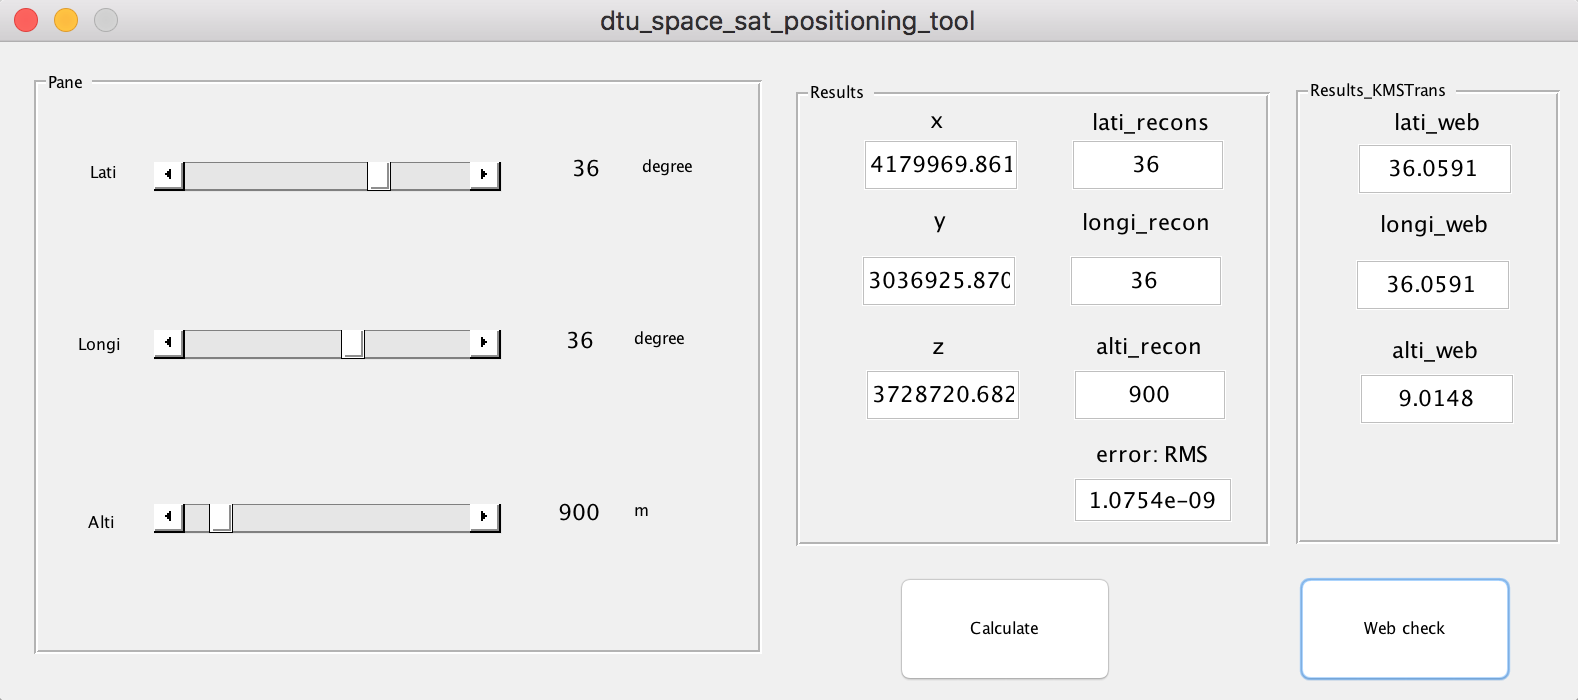
\includegraphics[width=\textwidth]{figures/gui.png}
	\caption{Snapshot of the designed GUI.}
	\label{fig:gui}
\end{figure}
\subsection{Conclusion}
Though various tests of my program, I believe that this program can correctly compute the coordinate transformation between the ECEF coordinate frame and the ellipsoidal coordinate frame. 
%\chapter{Assignment B: Satellite Coordinates from Kepler Elements}
The main objective of the assignment is to know how to compute and predict the satellites' position by using Kepler elements.

\section{Theory}
According to~\cite{misra2006global}, the orbital position of one satellite can be computed with
\begin{align}
	n &= \sqrt{\frac{GM}{a^3}} \\
	M & = n(t-t_p) \\
	M & = E-esinE \\
	\mathbf{r}&=\left[\begin{matrix}
		acosE-ae \\
		a\sqrt{1-e^2}sinE \\
		0 \\
	\end{matrix}\right]
\end{align}
where, $n$ is the mean motion, $GM$ is the earth's gravitational constant $3986004.418*10^8\ m/s^2$, $a$ is the length of the semi-major axis of ellipsoid ($6378137.0$ m), $e$ is the eccentricity of the ellipsoid calculated by $e^2=2f-f^2$ with $f$ being the flattening ($\frac{1}{298.257223563}$). \\
The transformation from the orbital coordinate frame to the ECEF coordinate frame can be computed using the inclination $i$, the right ascension of the ascending node $\Omega$ and the argument of perigee $\omega$.
\begin{equation}
\mathbf{r}_{ECEF}=\mathbf{R}(-\Omega)\mathbf{R}(-i)\mathbf{R}(-\omega)\mathbf{r}_{orbit}
\end{equation}

\section{Tasks}
\begin{itemize}
	\item Implement a \textsc{Matlab} function for estimating satellite positions in the orbital coordinate system.
	\item Convert the positions to the inertial system.
	\item Visualization of satellite positions for an interval.
\end{itemize}
\section{Code}
Complementary functions: \\
\textbf{deg2rad: conversion from degree to radian} as previous one. \\
\textbf{rad2deg: conversion from radian to degree} as previous one. \\
\textbf{consR: construct a rotation matrix}:
\lstinputlisting{../../assignment/utils/consR.m}
\textbf{estimateEccAnomaly: estimate eccentric anomaly}:
\lstinputlisting{../../assignment/utils/estimateEccAnomaly.m}
\textbf{lutOmegaAndAnomaly: lookup ascension and anomaly}:
\lstinputlisting{../../assignment/utils/lutOmegaAndAnomaly.m}
\textbf{calcSatPosition: compute satellite positions}:
\lstinputlisting{../../assignment/utils/calcSatPosition.m}
\textbf{ExampleHelperSat: visualization.}:
\lstinputlisting{../../assignment/ex2/ExampleHelperSat.m}
\textbf{Entry}:
\lstinputlisting{../../assignment/ex2/ex2_satellite_position_calc.m}
\begin{figure}[h]
	\centering
	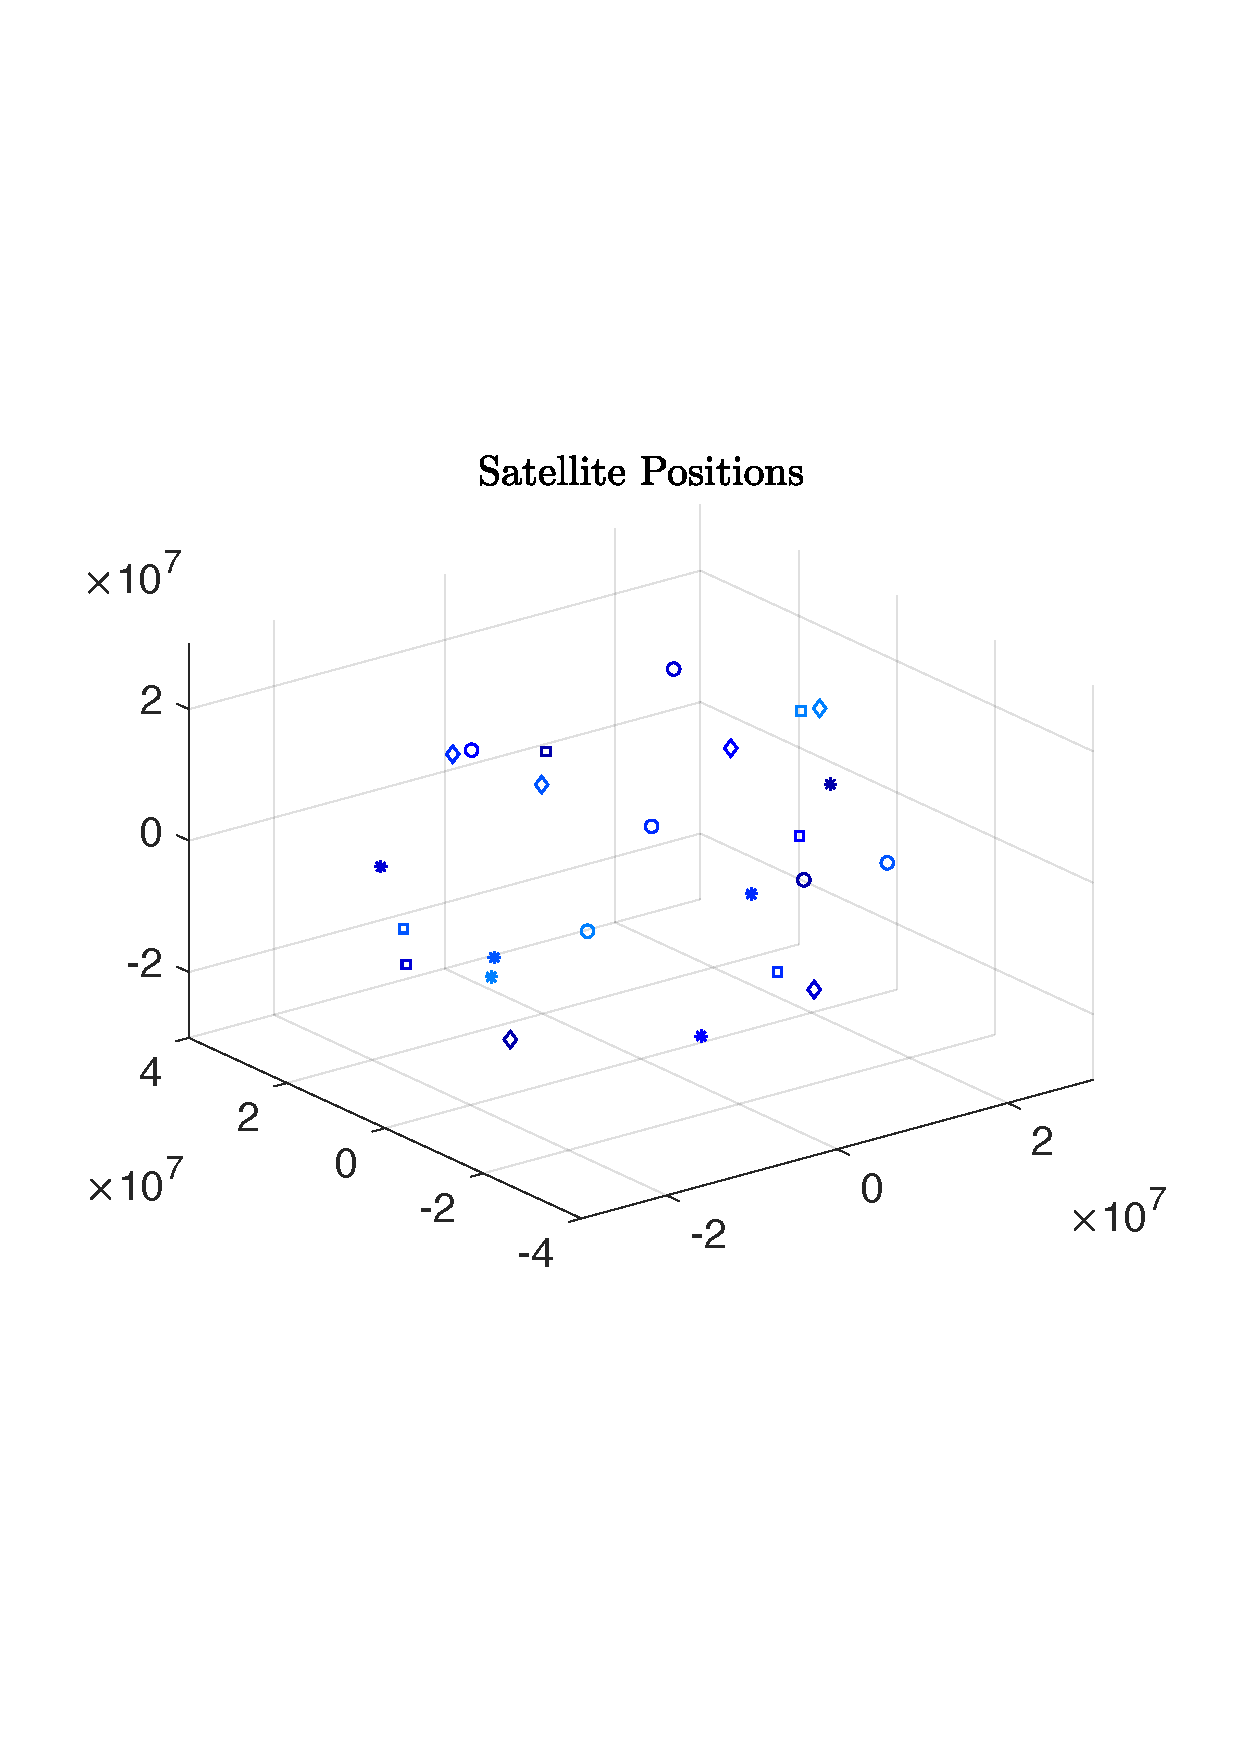
\includegraphics[width=\textwidth]{figures/ex21}
	\caption{Satellite Positions at given epoch.}
	\label{fig:ex2_1}
\end{figure}

\begin{figure}[h]
	\centering
	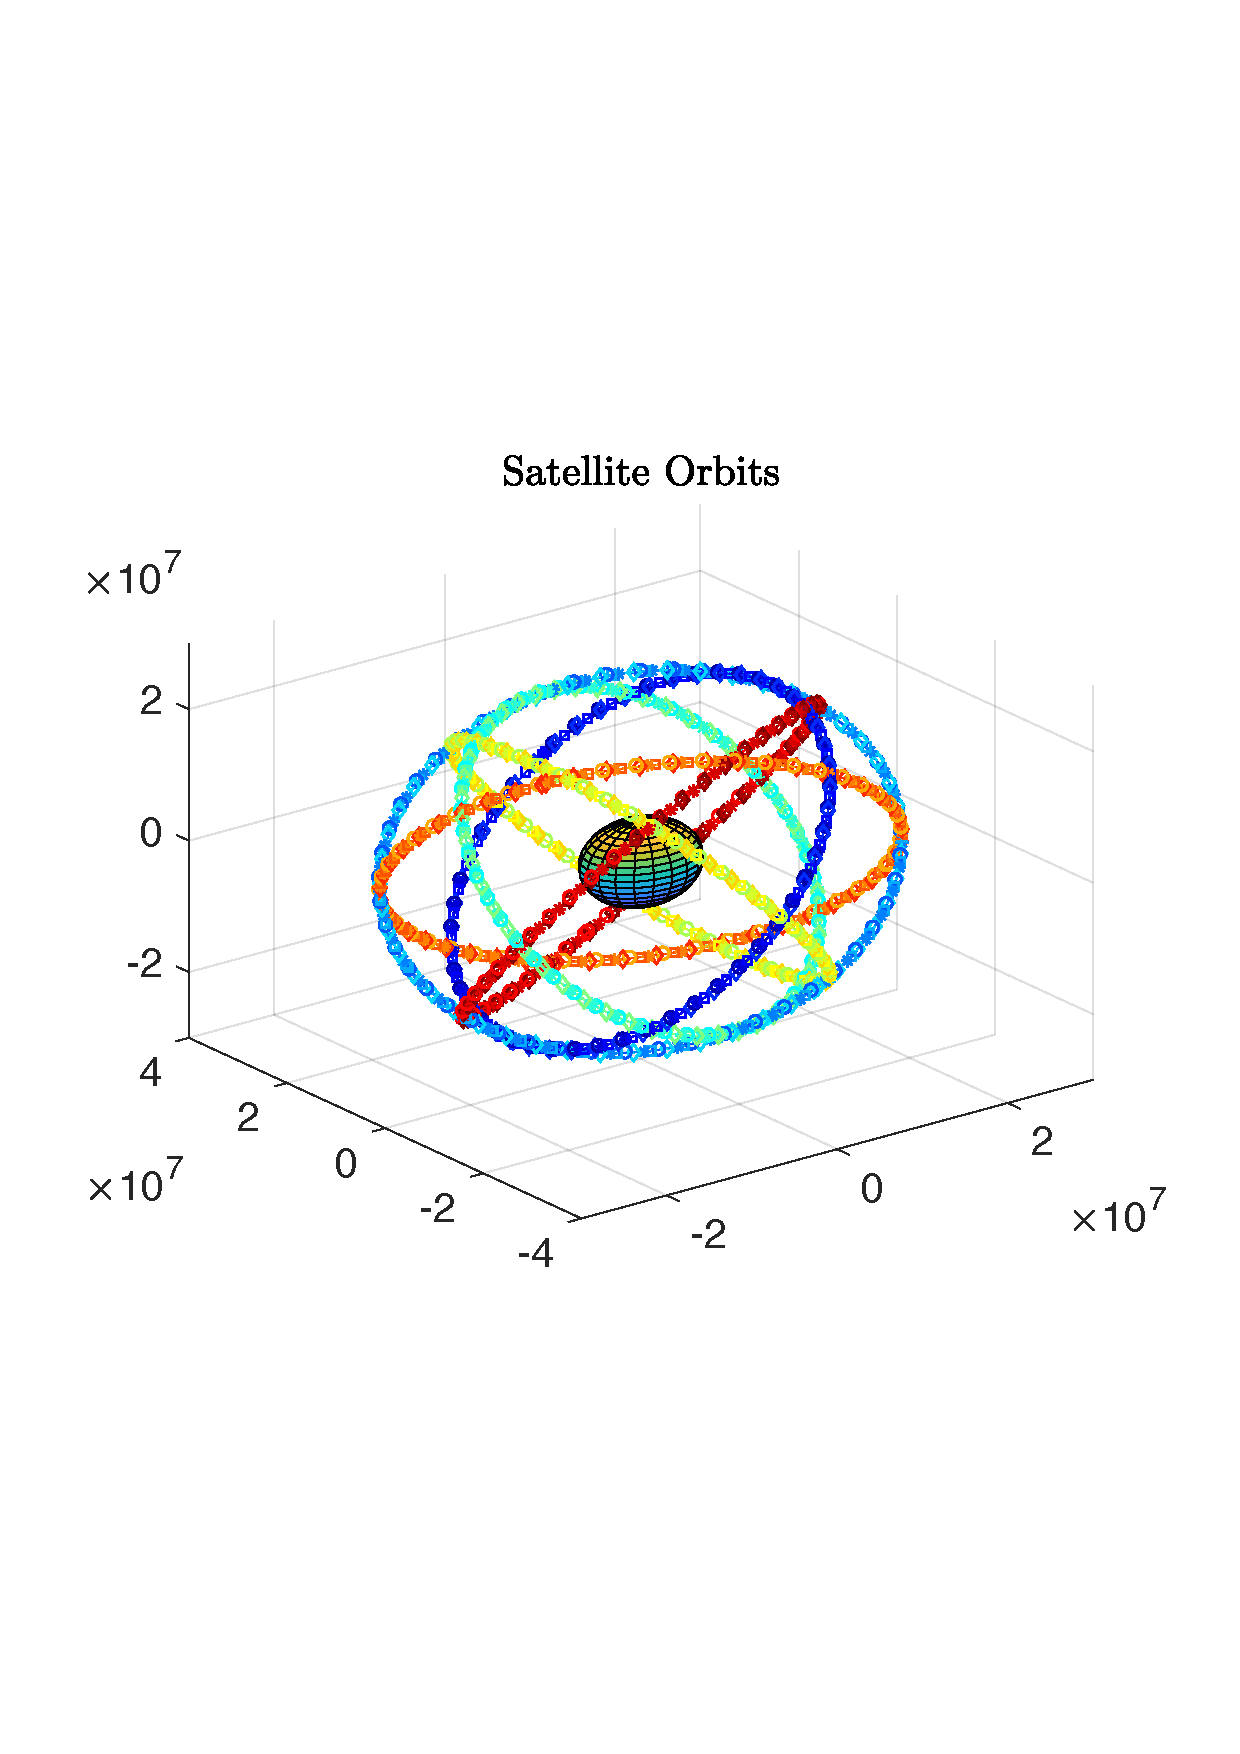
\includegraphics[width=.8\textwidth]{figures/ex22}
	\caption{Satellite orbits for 12 hours.}
	\label{fig:ex2_2}
\end{figure}
\section{Experiments}
\subsection{Single Epoch}
The result is shown in Fig~\ref{fig:ex2_1}
\subsection{Time Interval}
The result is shown in Fig~\ref{fig:ex2_2}
\subsection{DEMO Video}
A animation that demonstrates the motion of 24 satellites can be watched by the following link: \url{https://youtu.be/PjKFGVKaSvQ}.
\subsection{Conclusion}
Through this assignment, I grasp how to do the predictions of satellite positions using the Kepler elements.

%\chapter{Assignment C: Global and Local Coordinate Systems}
The main objective of the assignment is to grasp the transformation from the global coordinate system (WGS84) to the local East-North-Up (ENU) coordinate system. With this relationship, satellite positions can be projected to the local ENU coordinate system. Furthermore, the visibility of a given satellite can be determined by checking its elevation angle.

\section{Theory}
According to~\cite{misra2006global}, the transformation from the WGS84 frame to the ENU frame can be computed as:
\begin{align}
\left[\begin{matrix}
x_{ENU} \\
y_{ENU} \\
z_{ENU} \\
\end{matrix}\right] &= \mathbf{R}_{WGS84}^{ENU}
\left[\begin{matrix}
x_{WGS84} \\
y_{WGS84} \\
z_{WGS84} \\
\end{matrix}\right] \\
\mathbf{R}_{WGS84}^{ENU} &= \mathbf{R_1}(90^{\circ}-\phi)\mathbf{R_3}(90^{\circ}+\lambda) \\
\mathbf{R_1}(\alpha) &= 
\left[\begin{matrix}
1 & 0 & 0 \\
0 & cos(\alpha) & sin(\alpha) \\
0 & -sin(\alpha) & cos(\alpha) \\
\end{matrix}\right]\\
\mathbf{R_3}(\alpha) &= 
\left[\begin{matrix}
cos(\alpha) & sin(\alpha) & 0 \\
-sin(\alpha) & cos(\alpha) & 0 \\
0 & 0 & 1 \\
\end{matrix}\right]
\end{align}
Once the coordinates in the ENU frame is obtained, the azimuth, elevation, and zenith angles can be computed as follows:
\begin{align}
tan(\alpha_{azimuth}) &= \frac{x_{ENU}}{y_{ENU}} \\
cos(\alpha_{zenith}) &= \frac{z_{ENU}}{\sqrt{x_{ENU}^2+y_{ENU}^2+z_{ENU}^2}} \\
\alpha_{elevation} &= 90^{\circ}-\alpha_{zenith}
\end{align}
\section{Tasks}
\begin{itemize}
    \item Implement a \textsc{Matlab} function for transforming a point in the WGS84 frame to the local ENU frame.
	\item Implement a \textsc{Matlab} function that computes the azimuth, elevation and zenith angle.
	\item Read satellite positions for a given time epoch from a SP3 file and then convert the satellite positions to the ENU coordinates. Determine elevation and azimuth in the local coordinate system for the vectors to all GPS satellites at the given time epoch. Finally, determine the distances from origo to the satellites visible.
\end{itemize}
\section{Code}
Complementary functions: \\
\textbf{WGS842ENU: convert coordinates from WGS84 to ENU}:
\lstinputlisting{../../assignment/utils/WGS842ENU.m}
\textbf{calcAzimuthZenithElevation: compute the azimuth, zenith, elevation angle for a given point}:
\lstinputlisting{../../assignment/utils/calcAzimuthZenithElevation.m}
\textbf{sp3fileParser: parsing sp3 file.}:
\lstinputlisting{../../assignment/ex3/sp3fileParser.m}
\textbf{Entry}:
\lstinputlisting{../../assignment/ex3/ex3_enu_conversion.m}
\section{Experiments}
\subsection{Single Epoch}
The result is shown in Fig~\ref{fig:ex31}.
\begin{figure}[h]
	\centering
	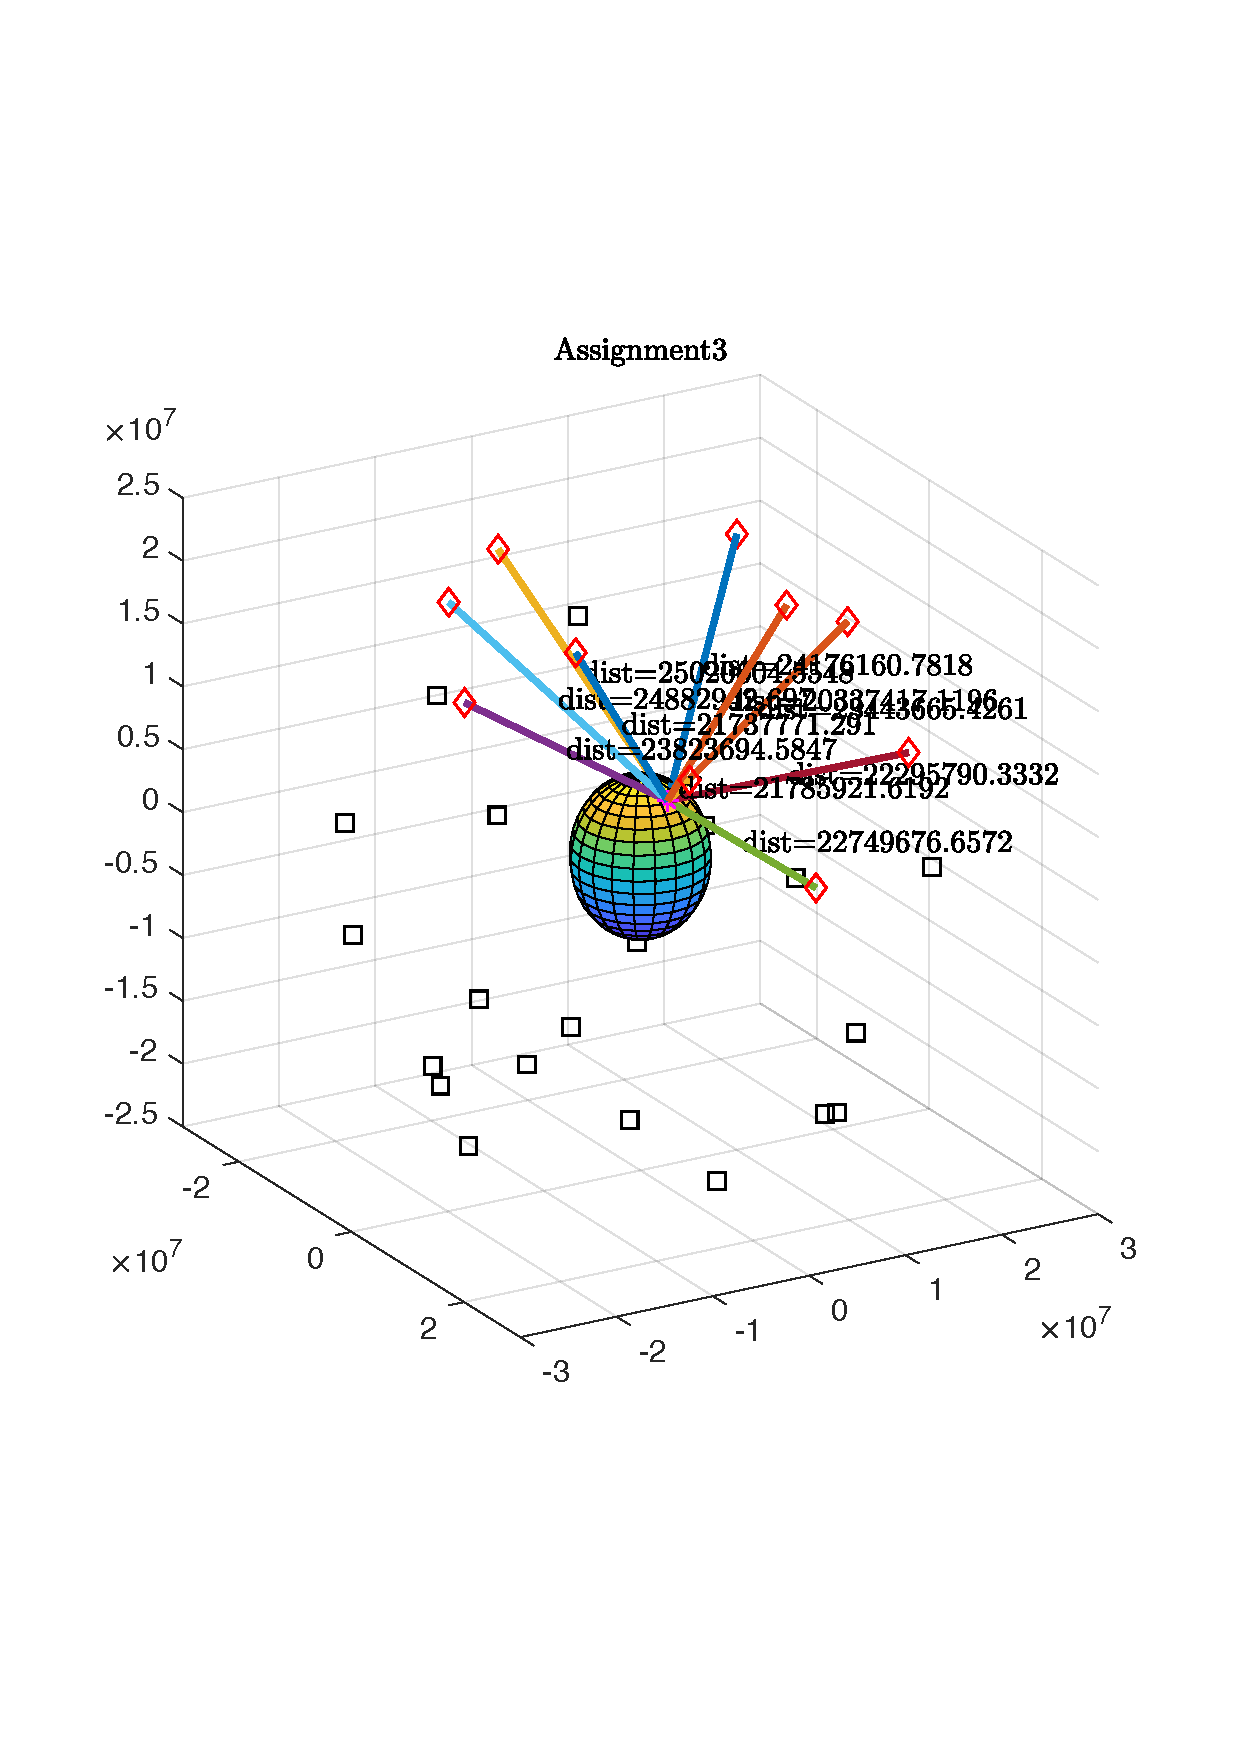
\includegraphics[width=\textwidth]{figures/ex31}
	\caption{Satellite visibili at a given epoch.}
	\label{fig:ex31}
\end{figure}
From the website of GPS.gov\footnote{\url{https://www.gps.gov/systems/gps/space/}}, it says that "GPS satellites fly in medium Earth orbit (MEO) at an altitude of approximately 20,200 km (12,550 miles)." Based on this data, it can be seen the calculated distances are reasonable since they are close to 20,200 km.

\subsection{Brute-force test}
In order to conveniently do more brute-force test, a \textsc{Matlab} GUI program is designed. The GUI program supports the following features:
\begin{enumerate}
	\item Automatically parse a sp3 file and list all relevant information.
	\item List all satellite positions' observations in a list box for the user to select.
	\item Input arbitrary latitude, longitude, and altitude.
	\item Visualization.
\end{enumerate}
Snapshots of the GUI program are shown as follows: \\
\textbf{Initialization}: \\
\begin{figure}[h]
	\centering
	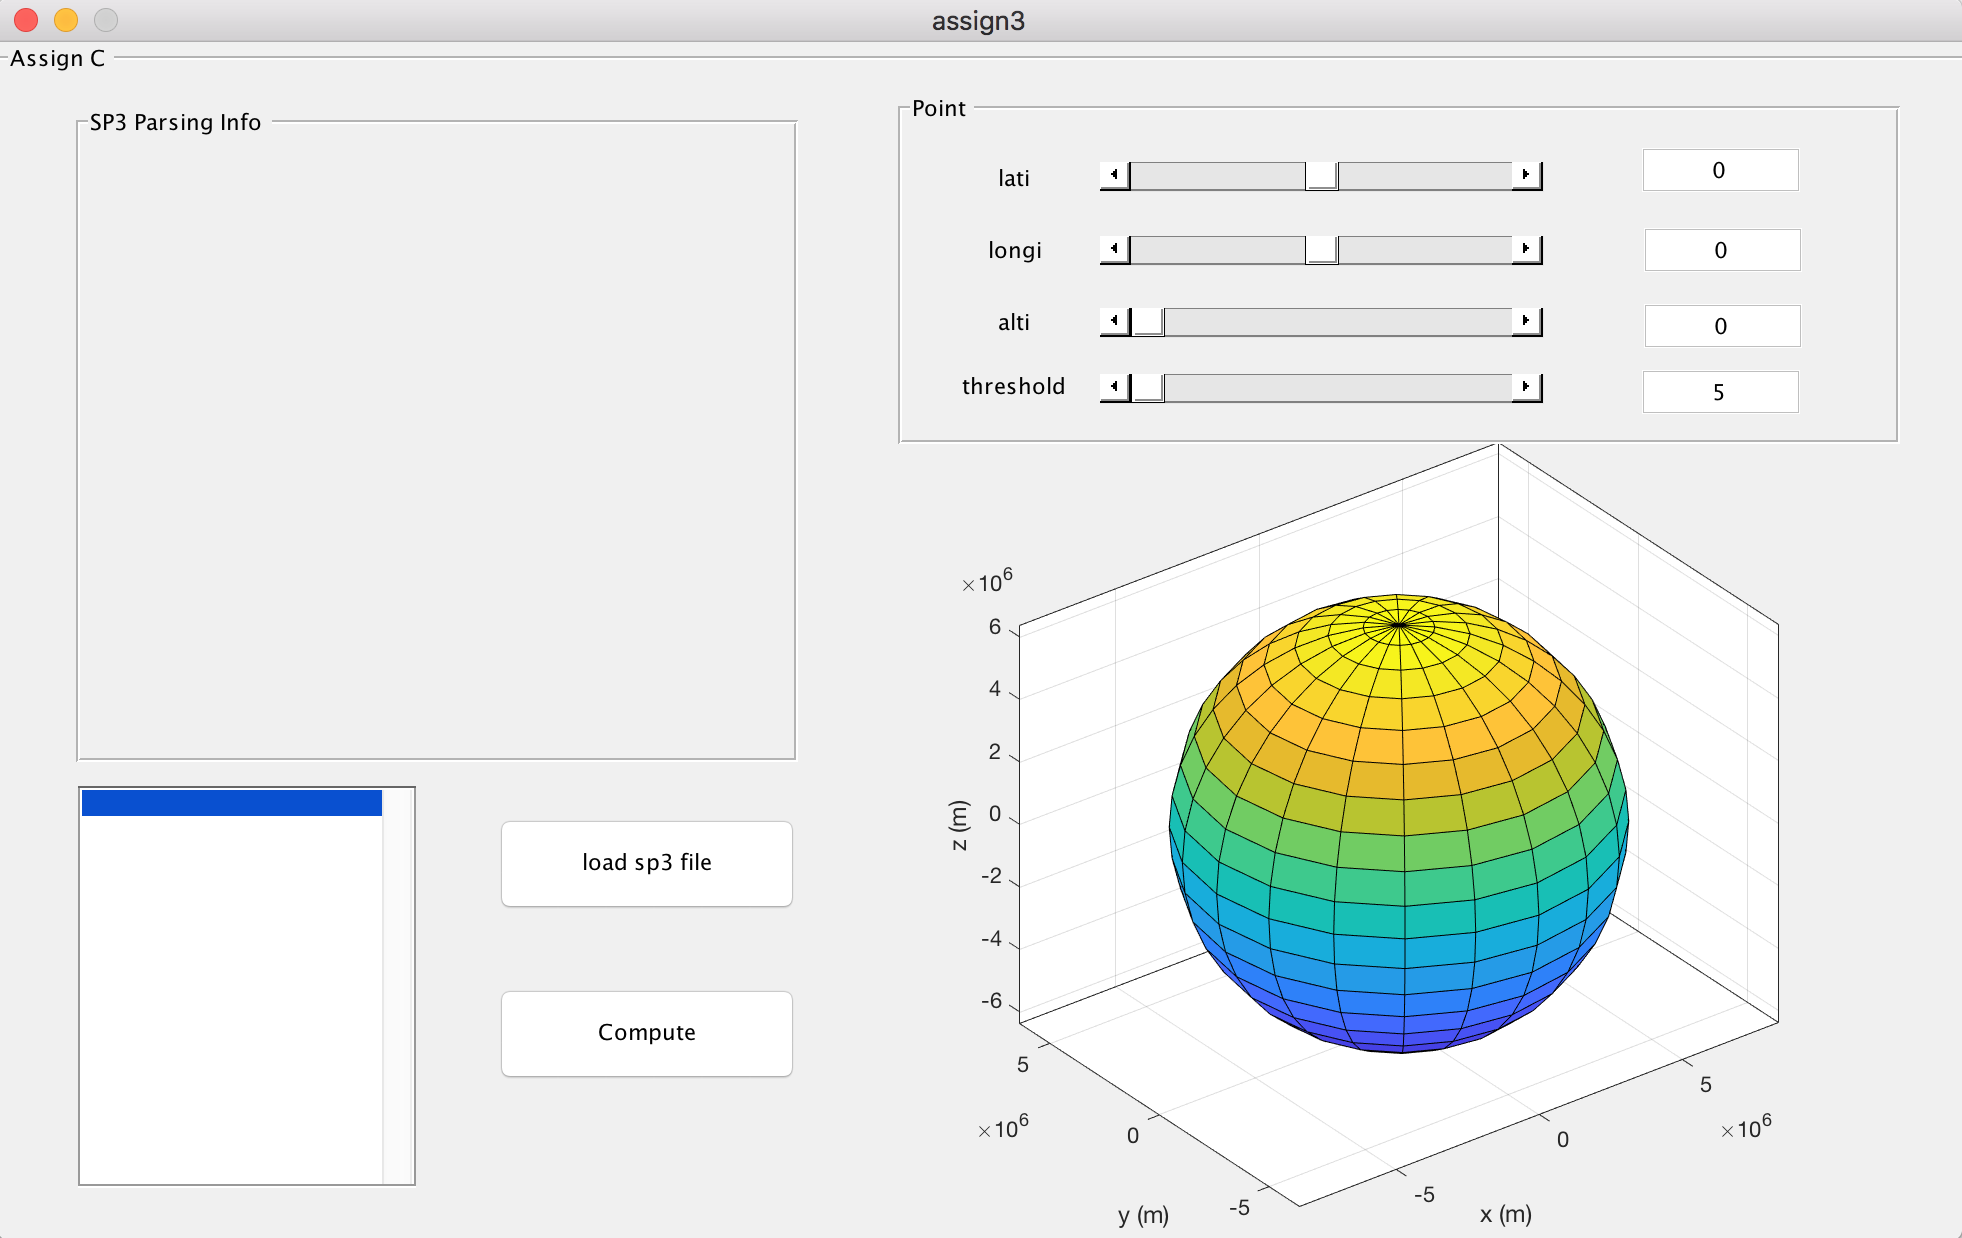
\includegraphics[width=\textwidth]{figures/ex3init}
	\caption{Initialization.}
\end{figure}
\textbf{After loading a sp3 file}: \\
\begin{figure}[h]
	\centering
	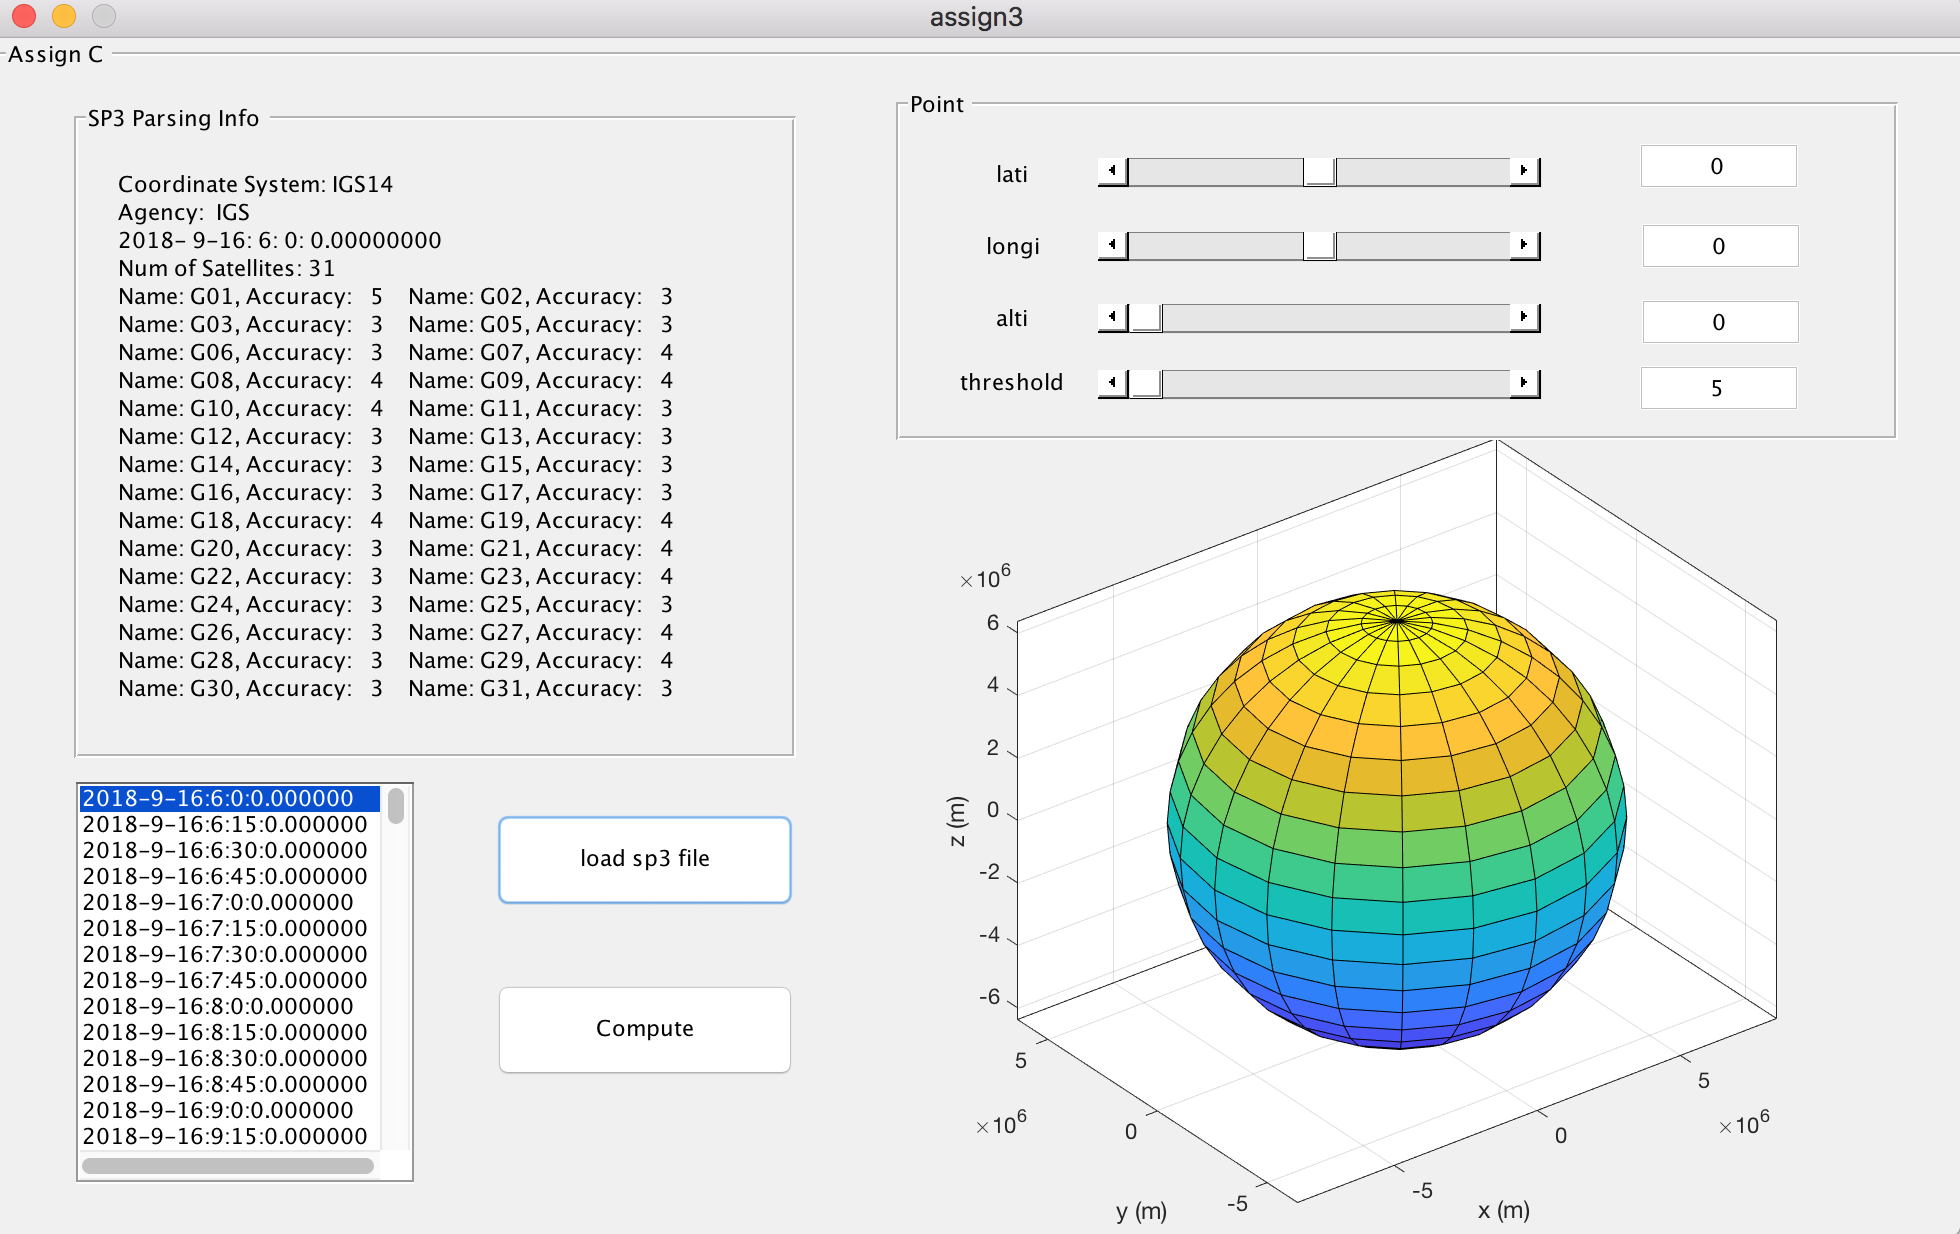
\includegraphics[width=\textwidth]{figures/ex3loadsp3}
	\caption{Loading a sp3 file.}
\end{figure}
\textbf{Results of 2 examples}: \\
\begin{figure}[h]
	\centering
	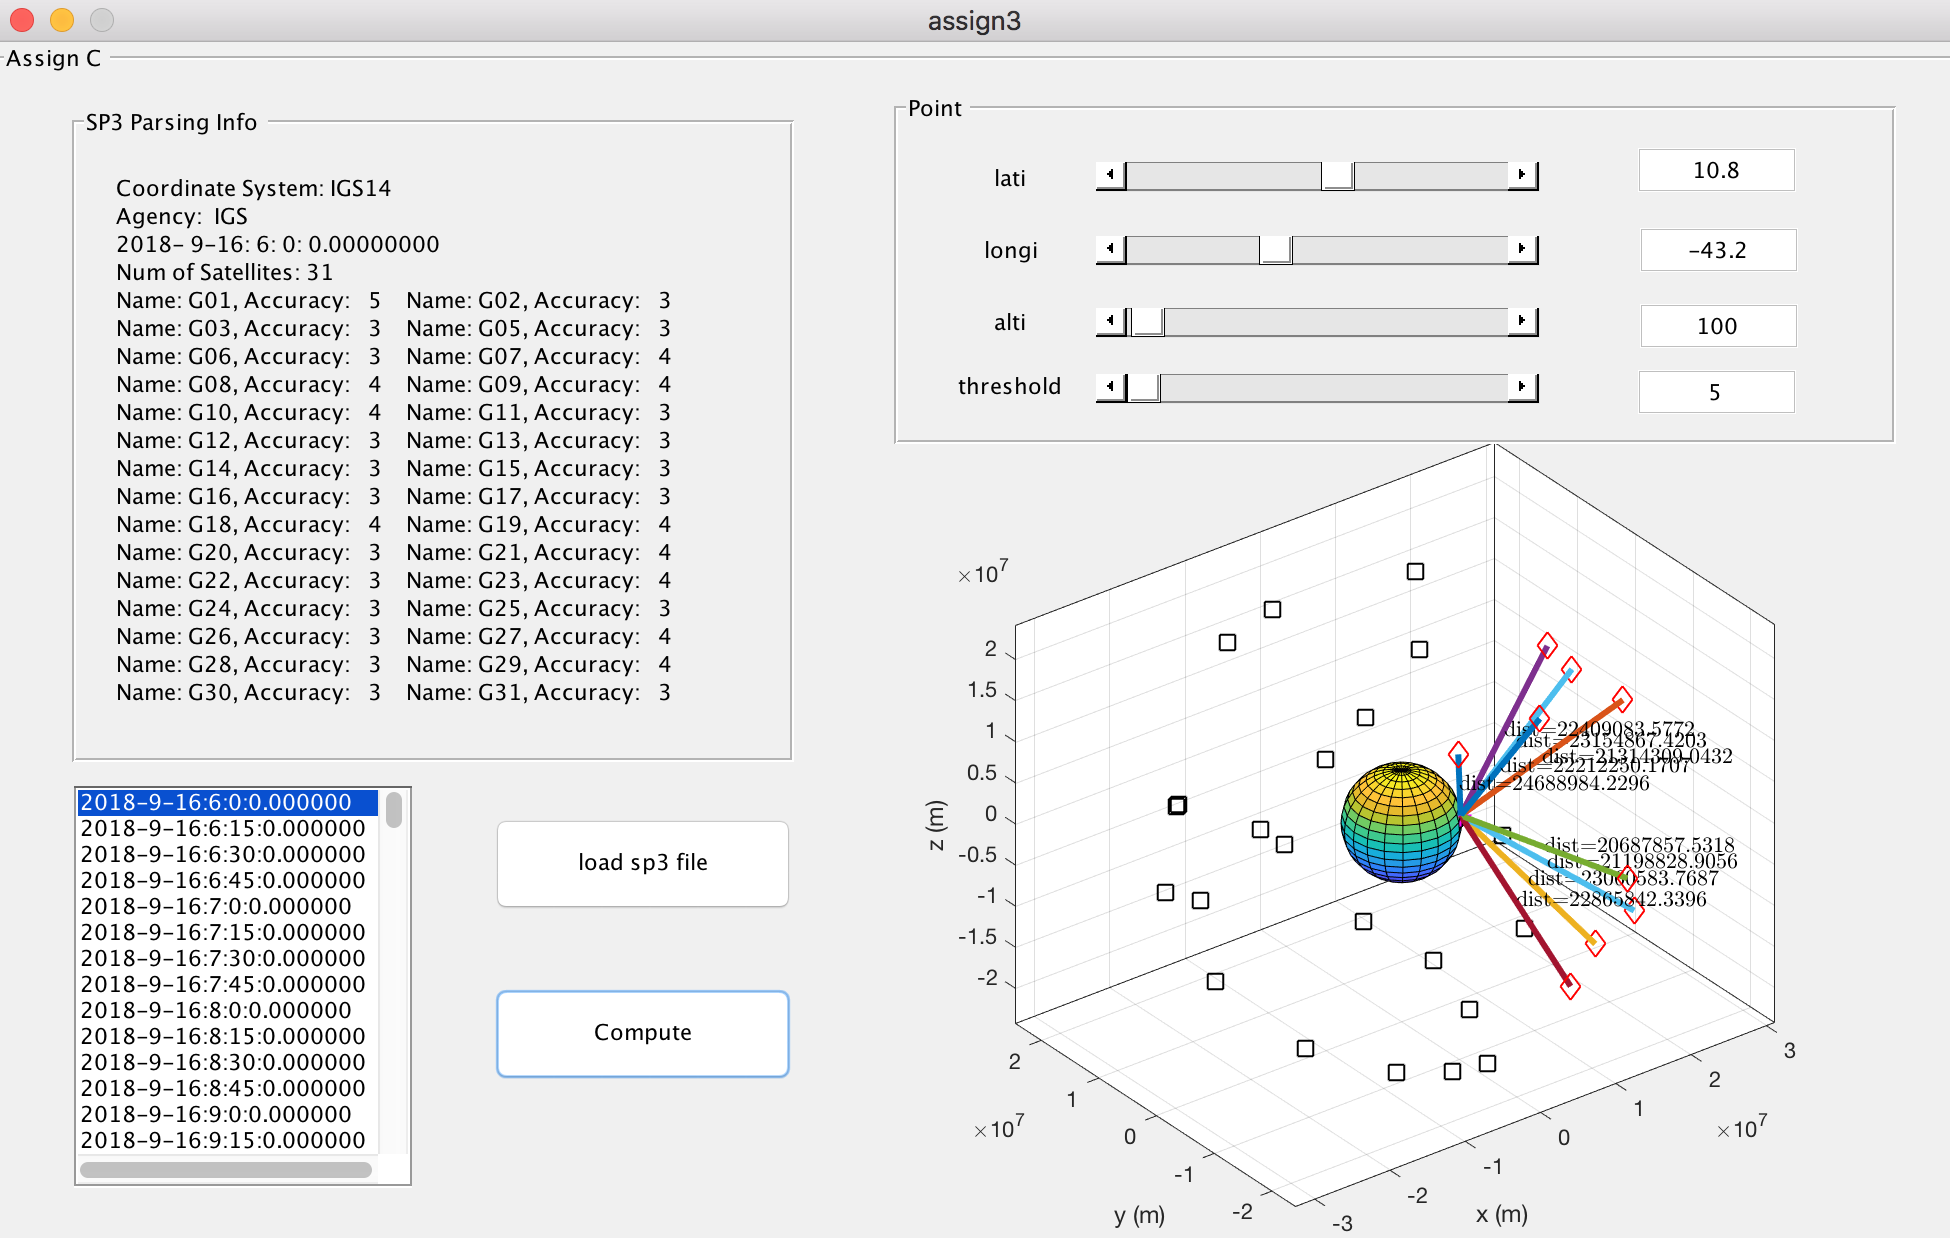
\includegraphics[width=\textwidth]{figures/ex3com1}
	\caption{Snapshot of the result 1.}
\end{figure}
\begin{figure}[h]
	\centering
	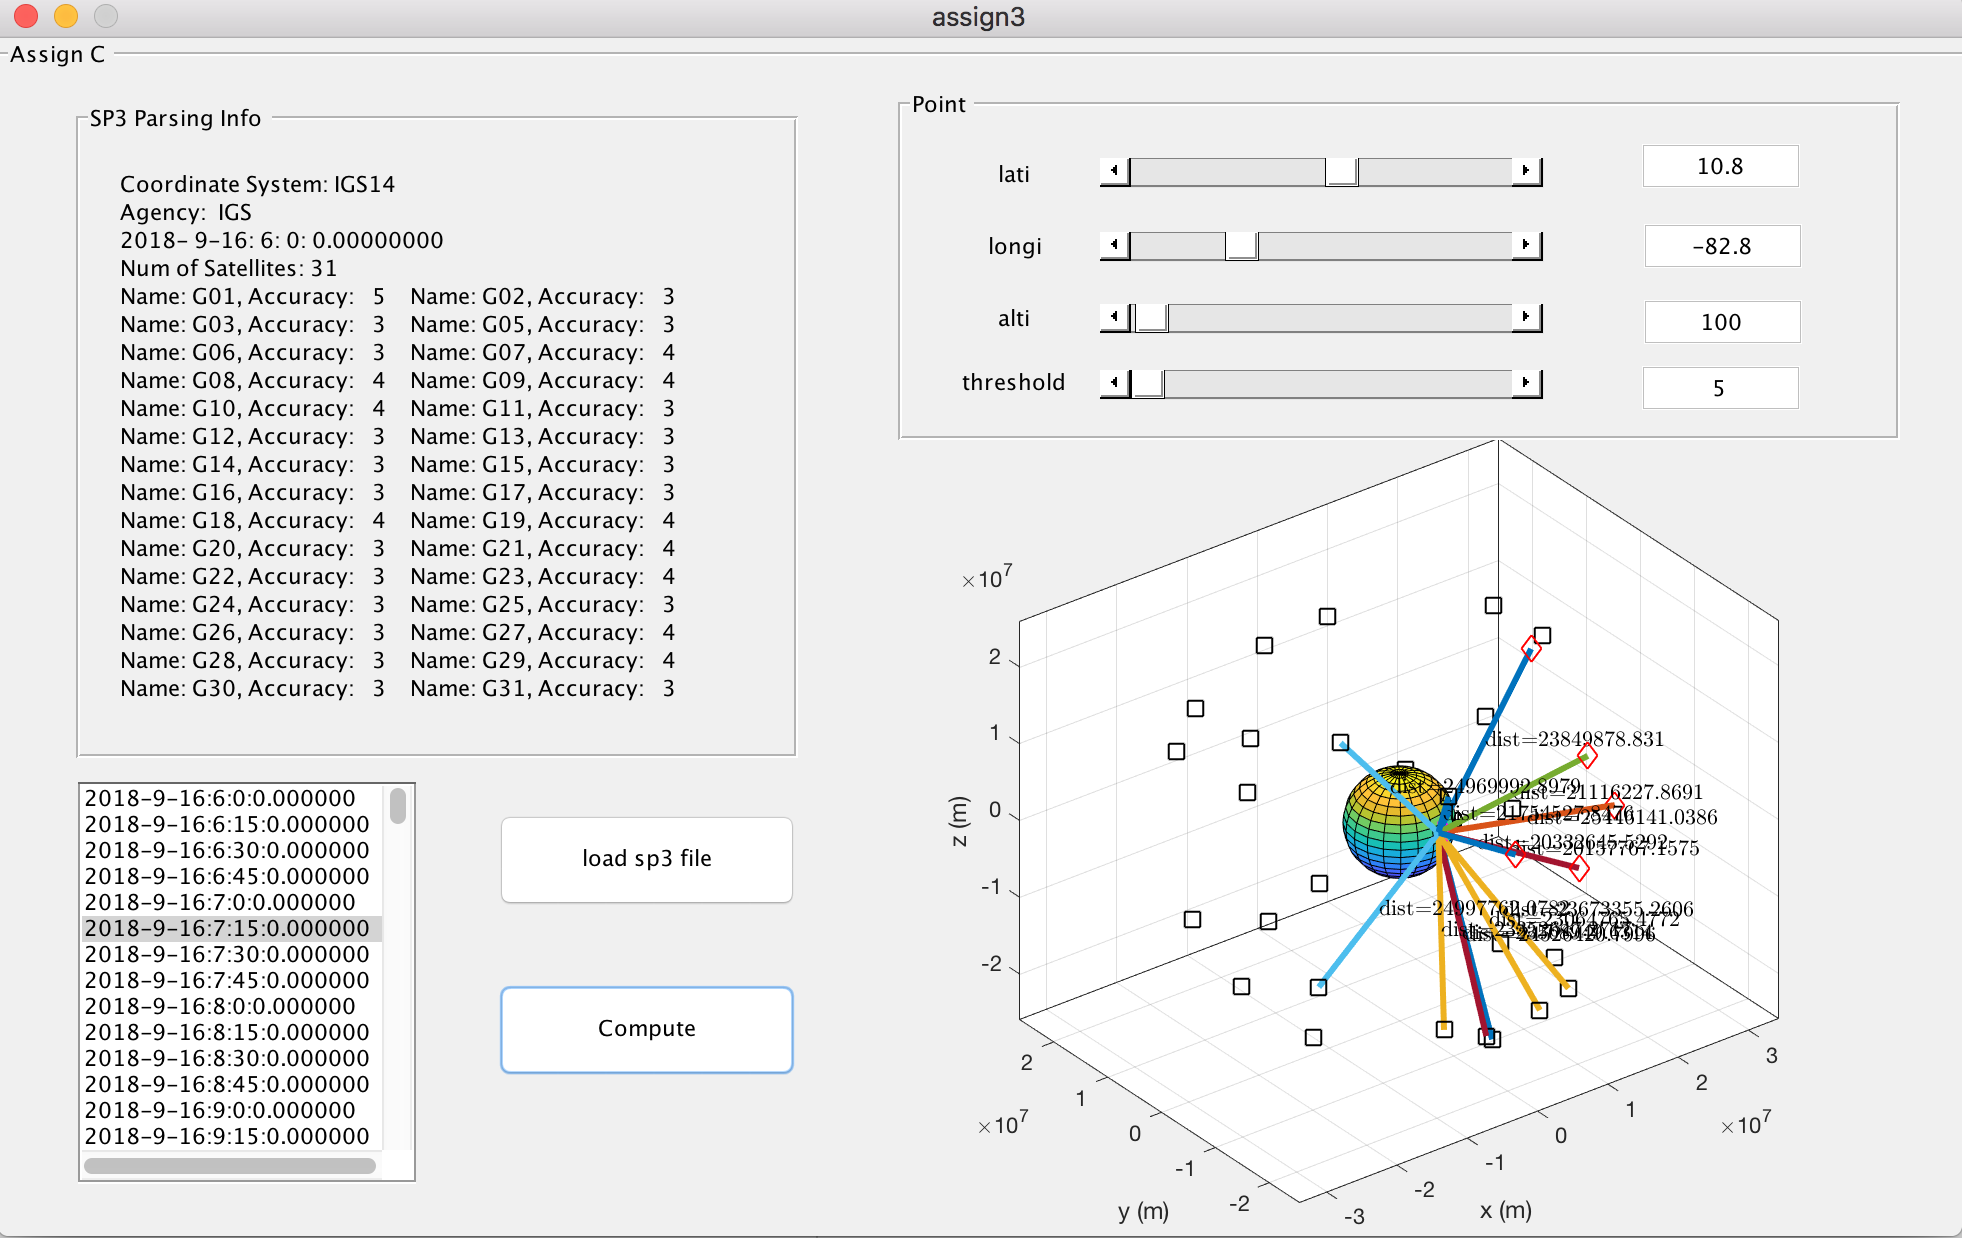
\includegraphics[width=\textwidth]{figures/ex3com2}
	\caption{Snapshot of the result 2.}
\end{figure}
\subsection{Conclusion}
Through this assignment, I grasp how to do the conversion from WGS84 to ENU frame and verify the visibility of a given satellite by checking its elevation angle. \\
I designed a GUI program that can easily parse a sp3 file, and do the conversion automatically. The program is easy-to-use.
%\include{files/assign_d}
%\include{files/assign_e}
\include{files/assign_f}

%\include{files/reportWriting}
%\chapter{Layout and use of the template }
This chapter describes how to use the template for the report. The template is set up as the format the report should meet and is used at Center for electric power and energy. Please do not change the setup of the template, styles etc.. A frequent problem when using the template is corruption in the text close to the headline and the headlines. Read more on this in chapter 3.4.

\FloatBarrier
\input{files/3.1}
\FloatBarrier
\input{files/3.2}
\FloatBarrier
\input{files/3.3}
\FloatBarrier
\input{files/3.4}
\FloatBarrier
\input{files/3.5}
\FloatBarrier
\section{Figures}
To insert a figure, go to Insert Picture/From File, locate and select a picture, and choose the method of insertion. Please turn off any Float Over Text feature; figures should al-ways be in line with text.

After the figure has been placed, it needs a Figure number and a Caption:
\begin{itemize}
	\item Hit return once to place the cursor under the figure
	\item Hit the button Insert Caption Figure to insert figure numbering. In appendices use the button Insert Caption Figure Appendix instead
	\item Do not modify figure numbering to include additional characters such as Figure 2-1(a), or Figure 2-1(a), as the List of Figures will not work properly. If you want to include sub-numbers include them under one common figure caption, e.g.: “Figure 2-1: (a) Text. (b) Text.”.
\end{itemize}

You can create cross-references using this button in the toolbar report. This is for example, a cross-reference to Figure 3.1.

\begin{figure}[h]
	\centering
	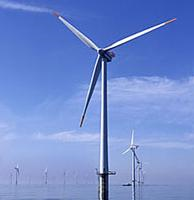
\includegraphics[scale=1]{figures/windmill.png}
	\caption{Write a self-explaining caption. Captions are important for the reports readability}
	%\label{my-label}
\end{figure}

\begin{minipage}{0.5\textwidth}

\begin{figure}[H]
	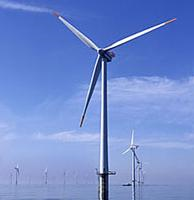
\includegraphics[scale=1]{figures/windmill.png}
	\caption{Example of two figure alligned side by side. Use a table as shown }
	%\label{my-label}
\end{figure}
\end{minipage} \hfill
\begin{minipage}{0.47\textwidth}
\begin{figure}[H]
	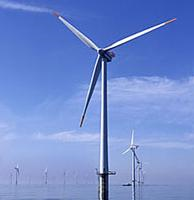
\includegraphics[scale=1]{figures/windmill.png}
	\caption{Example of two figures alligned side by side}
	%\label{my-label}
\end{figure}

\end{minipage}

Below with a vertical setup writing the Title above and the text describing the figure below.
\FloatBarrier
\section{Tables}
Use the style for the tables as in the example shown below. 

To insert a table text, use the button Insert Caption Table. In the appendix, you may use the button Insert Caption Table Appendix. Table text is inserted immediately above the table. 

You can make cross-references using this button in the toolbar. This is, for example, a cross-reference to Table 3.4

\begin{table}[h]
\centering
\caption{Write a short self-explaining text}
%\label{my-label}
\begin{tabular}{|l|l|}
\hline
\textbf{Title} & \textbf{Title} \\ \hline
Table body     & Table body     \\ \hline
Table body     & Table body     \\ \hline
\end{tabular}
\end{table}


\begin{table}[h]
\centering
\caption{Write a short self-explaining text}
%\label{my-label}
\begin{tabular}{|l|l|l|l|}
\hline
\textbf{Title} & \textbf{Title} & \textbf{Title} & \textbf{Title} \\ \hline
Table body     & Table body     & Table body     & Table body     \\ \hline
Table body     & Table body     & Table body     & Table body     \\ \hline
Table body     & Table body     & Table body     & Table body     \\ \hline
\end{tabular}
\end{table}

\FloatBarrier
\section{Equations}
Equations should be indented by 0.75 cm. Equations are numbered on the right side with a number enclosed in brackets. The formula number shall consist of a chapter num-ber and serial number separated by a period. This is handled by using the Insert button in the Equation toolbar. 

You can make cross-references to equations using this button in the tool bar. This is, for example, a cross-reference to equation (3.1). 

The following are examples of equations:

\begin{align}
Y=\sum_{i}\frac{4k_i}{X_i} \\
Y=\sum_{i}\frac{4k_i}{X_i}
\end{align}
\FloatBarrier
\input{files/3.9}
\FloatBarrier
%\include{files/reportHandin}
%\chapter{Conclusion}
A In this chapter the conclusion is written. It can contain the following chapters.

\section{Results}
Use his chapter for a brief description of the main results, which have been achieved. Remember only to mention results which have not been mentioned prior. 


\section{Perspectives}
Describe the results in a broader perspective, e.g.: What validity of the results is ex-pected under other conditions? How do the report's findings impact the situation in a larger perspective? How does this work with other activities and results?


\section{Future work}
Describe the work, which is estimated as necessary to obtain further results with the described problem. Are there spin-offs, which are important. Are there areas, which are only sparsely cowered and have to undergo further research. Is it possible to look into an entirely different method?




% in documenet


%%%%% BIBLIOGRAPHY %%%%% 
\begingroup
	\raggedright
	\bibliography{bibtex/litteratur}
\endgroup


%%%%% APPENDICES %%%%%
%\newpage\thispagestyle{empty}\mbox{}
%\begin{appendices}
%	\chapter{Write appendix heading here}
The appendix can be written here.

\begin{figure}[h]
	\centering
	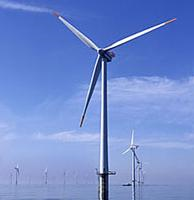
\includegraphics[scale=1]{figures/windmill.png}
	\caption{Write a self-explaining caption. Captions are important for the reports readability}
	%\label{my-label}
\end{figure}

It is possible to insert both figures and tables in the appendix.

\begin{table}[h]
\centering
\caption{write a short text for the figure, which is self-explaining}
%\label{my-label}
\begin{tabular}{|l|l|}
\hline
\textbf{Title} & \textbf{Title} \\ \hline
Table body     & Table body     \\ \hline
Table body     & Table body     \\ \hline
\end{tabular}
\end{table}

Following equation has been utilized in the appendix:
\begin{align}
R=5~\Omega
\end{align}
%	\chapter{Write appendix heading here}
The appendix can be written here.
%\end{appendices}




	\thispagestyle{empty}
	\enlargethispage{1.3cm}
	\calccentering{\unitlength}
	\begin{adjustwidth}{\unitlength}{-\unitlength}
		\vspace*{-1.9cm}
		\begin{raggedright}
			\vspace{\stretch{2}}
		\end{raggedright}
		\begin{raggedright}
		\noindent\deptname
		\vspace{\stretch{0.01}} 
		\noindent\addressname
		\noindent \url{www.space.dtu.dk}\\ 
		\noindent \newline
		%\noindent Tel: (+45) 45 25 35 00 \\
		%\noindent Fax: (+45) 45 88 61 11\\ 
		\noindent E-mail:~\url{xiahaa@space.dtu.dk}
		\vspace{0.5cm}\\
		%Write ISBN XX-XXXXX-XX-X (or delete)
		\end{raggedright}
	\end{adjustwidth}



	
	 				
\end{document}